\begin{minipage}{0.45\textwidth}

\paragraph{Activité~1} Retrouvez les vecteurs égaux.

\begin{center}
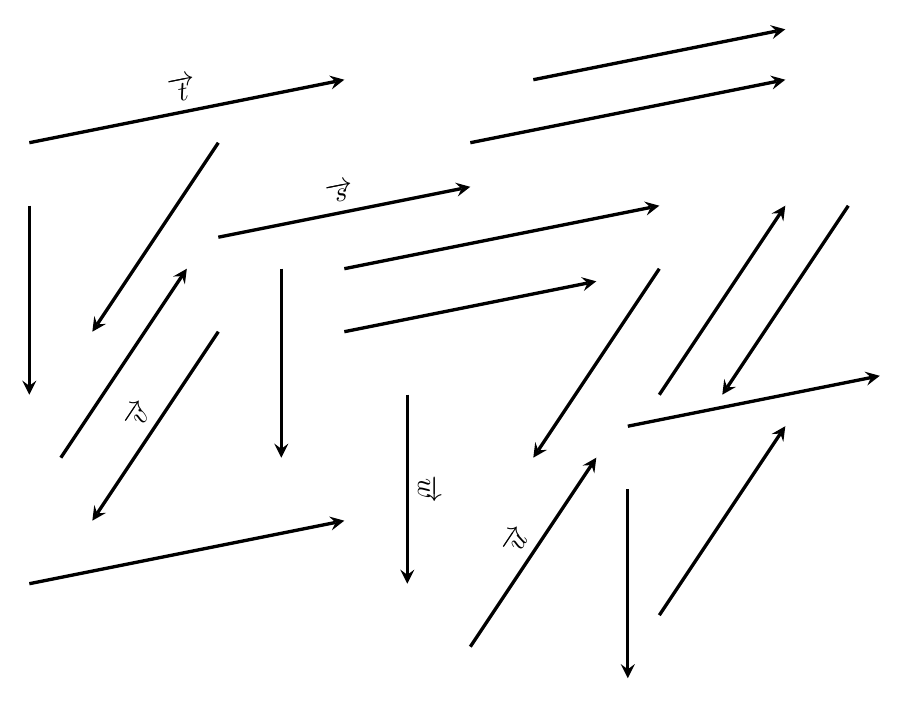
\begin{tikzpicture}[scale=0.8,every node/.style={scale=1}]
	\tikzstyle{vect}=[->,>=stealth,very thick]
	\tikzstyle{vectred}=[vect]
	\tikzstyle{vectblue}=[vect]
	\tikzstyle{vectgreen}=[vect]
	\tikzstyle{vectgray}=[vect]
	\tikzstyle{vectcyan}=[vect]
	

\coordinate (A) at (2,2);
\coordinate (B) at (5,6);
\coordinate (C) at (-4.5,5);
\coordinate (D) at (5,2.5);
\coordinate (u) at (2,3);
\draw[vectred] (A) -- ++ (u) node[midway, sloped, above]{$\overrightarrow{u}$};
\foreach \point in {B, C, D}
	\draw[vectred] (\point) -- ++ (u);

\coordinate (E) at (-2,7);
\coordinate (F) at (-2,10);
\coordinate (G) at (8,9);
\coordinate (H) at (5,8);
\coordinate (v) at (-2,-3);
\draw[vectblue] (E) -- ++ (v) node[midway, sloped, above]{$\overrightarrow{v}$};
\foreach \point in {F, G, H}
	\draw[vectblue] (\point) -- ++ (v);

\coordinate (I) at (1,6);
\coordinate (J) at (-1,8);
\coordinate (K) at (4.5,4.5);
\coordinate (L) at (-5,9);
\coordinate (w) at (0,-3);
\draw[vectgreen] (I) -- ++ (w) node[midway, sloped, above]{$\overrightarrow{w}$};
\foreach \point in {J, K, L}
	\draw[vectgreen] (\point) -- ++ (w);

\coordinate (M) at (-5,10);
\coordinate (N) at (-5,3);
\coordinate (O) at (0,8);
\coordinate (P) at (2,10);
\coordinate (t) at (5,1);
\draw[vectgray] (M) -- ++ (t) node[midway, sloped, above]{$\overrightarrow{t}$};
\foreach \point in {N, O, P}
	\draw[vectgray] (\point) -- ++ (t);

\coordinate (Q) at (-2,8.5);
\coordinate (R) at (4.5,5.5);
\coordinate (S) at (0,7);
\coordinate (T) at (3,11);
\coordinate (s) at (4,0.8);
\draw[vectcyan] (Q) -- ++ (s) node[midway, sloped, above]{$\overrightarrow{s}$};
\foreach \point in {R, S, T}
	\draw[vectcyan] (\point) -- ++ (s);
\end{tikzpicture}
\end{center}

\paragraph{Activité~3} Complétez les égalités suivantes~:\\
%\begin{center}
\begin{minipage}{0.5\textwidth}
\begin{tikzpicture}[scale=0.75,every node/.style={scale=1}]
	\tikzstyle{vect}=[->,>=stealth,ultra thick]
	
	\clip (-1,-1) rectangle (5,5);
	\placerpoint{A}{1}{2}{above left}
	\placerpoint{B}{2}{3}{above left}
	\placerpoint{C}{3}{2}{above right}
	\placerpoint{D}{2}{1}{below left}
	\draw (A) -- (B) -- (C) -- (D) -- cycle;
	\draw[vect] (A) -- (B);
	\draw[vect] (B) -- (C);
	\draw[vect] (A) -- (D);
	\draw[vect] (D) -- (C);
	\draw (0,0) grid (4,4);
\end{tikzpicture}
\end{minipage}
\begin{minipage}{0.5\textwidth}
\vectaffiche{AB} + \vectaffiche{BC} = \\
\vectaffiche{AD} + \vectaffiche{DC} = \\[1em]
\vectaffiche{AD} + \vectaffiche{CB} + \vectaffiche{AB} = \\
\end{minipage}

\begin{minipage}{0.5\textwidth}
\begin{tikzpicture}[scale=0.75,every node/.style={scale=1}]
	\tikzstyle{vect}=[->,>=stealth,ultra thick]
	
	\placerpoint{E}{0}{2}{above left}
	\placerpoint{F}{2}{4}{above left}
	\placerpoint{G}{4}{2}{above right}
	\placerpoint{H}{2}{0}{below left}
	\draw (E) -- (F) -- (G) -- (H) -- cycle;
	\draw[vect] (E) -- (F);
	\draw[vect] (F) -- (G);
	\draw[vect] (E) -- (H);
	\draw[vect] (H) -- (G);
	\draw (-1,-1) grid (5,5);
\end{tikzpicture}
\end{minipage}
\begin{minipage}{0.5\textwidth}
\vectaffiche{EF} + \vectaffiche{FH} + \vectaffiche{HG} = \\
\vectaffiche{EH} + \vectaffiche{HF} + \vectaffiche{FG} = \\[1em]
\vectaffiche{EG} + \vectaffiche{FE} = \\
\vectaffiche{EH} + \vectaffiche{EF} = \\[1em]
\vectaffiche{FH} + \vectaffiche{EF} = \\
\vectaffiche{GE} + \vectaffiche{FG} + \vectaffiche{EF} = \\[1em]
\end{minipage}



\vspace{-4em}


\end{minipage}
\newpage

\begin{minipage}{0.45\textwidth}
\thispagestyle{activite}

\paragraph{Activité~2} ~\\

%\section{Définitions}

%\vfill
\begin{center}
\begin{tikzpicture}[scale=0.8,every node/.style={scale=0.7}]
	\tikzstyle{vect}=[->,>=stealth,very thick]
%	\clip (0.1,0.1) rectangle (14.9,9.9);
	\grille{0}{0}{15}{10}{help lines};
	\vect{A}{B}{2}{4}{3}{8}{left}{right}{red};
%	\vect{C}{D}{4}{6}{4}{2}{above}{below}{red};
	\vect{C}{D}{11}{8}{14}{9}{left}{right}{red};
	\vect{E}{F}{14}{1}{12}{4}{right}{left}{red};
	\placerpoint{M}{7}{3}{left}
%	\draw[vect,red,line width=1.5pt] (M) -- ++ (3,1);
%	\draw[vect,red,line width=1.5pt] (M) ++ (3,1) -- ++ (-2,3);
%	\draw[vect,<-,red,line width=1.5pt] (M) ++ (3,1) ++ (-2,3) -- (M);
\end{tikzpicture}
\end{center}

\begin{enumerate}
	\item Sur la figure ci-dessus, placer N image de M par la translation qui envoie C en D.
	\item Ensuite, placer O image de N par la translation qui envoie E en F.
	\item Que peut on dire de $\overrightarrow{AB}$ et de $\overrightarrow{MO}$~?
	\item Quelle est la nature du quadrilatère ABOM~?
\end{enumerate}
%\end{center}

\end{minipage}